\documentclass{utsignal}

\usepackage{amsmath}
\usepackage{wrapfig}
\usepackage{verbatim}
\usepackage{fancyvrb}
\usepackage{lscape}
\usepackage{rotating}
\usepackage{xepersian}
\usepackage{listings}
\usepackage{color}
\usepackage[utf8]{inputenc}

\title{تمرین کامپیوتری شماره‌ی ۱}
\course{سیگنال‌ها و سیستم‌ها}
\author{\href{mailto:hodabpour@gmail.com?subject=[SS\%20S98 A1]}{هدی برخوردارپور}، 
\href{mailto:ranjbar.ali@ut.ac.ir?subject=[SS\%20S98 A1]\%20}{علی رنجبر}}
\lecturer{امیرمسعود ربیعی}
\deadline{چهارشنبه ۲۲ اسفند ۱۳۹۷، ساعت ۲۳:۵۵}
\graphicspath{{./img/}}


\begin{document}
    \maketitle
    \section{مقدمه}
        در این تمرین کامپیوتری قصد داریم با نرم‌افزار ‌‌متلب\LTRfootnote{MATLAB}  و متمتیکا\LTRfootnote{Mathematica} آشنا شویم.
    \subsection{متلب}
 متلب، یک محیط نرم‌افزاری برای انجام محاسبات عددی و یک زبان برنامه‌نویسی نسل چهارم است که از ترکیب دو واژهٔ MATrix (ماتریس) و LABoratory (آزمایشگاه) ایجاد شده‌است.  این نام حاکی از رویکرد ماتریس محور برنامه است، که در آن حتی اعداد منفرد هم به عنوان ماتریس در نظر گرفته می‌شوند.
    \subsection{متمتیکا}
    متمتیکا، یک نرم‌افزار جبری بسیار رایج، که توسط شرکت ولفرم ریسرچ پدید آورده شده است و اکثر توابع نرم‌افزاری موردنیاز در ریاضی و علوم طبیعی را در اختیار استفاده‌کنندگان آن قرار می‌دهد.
    \subsection{مقایسه‌ی متلب و متمتیکا}
    \begin{itemize}
        \item جهت‌گیری متلب بیشتر برای کار با داده هاست (که در این بسیار خوب عمل می‌کند) اما با اینکه امکان محاسبات نمادین در‌ متلب وجود دارد، این امکان در متمتیکا بسیار آسان‌تر و کارآمدتر است. 
        \item متلب یک محیط برنامه‌نویسی در حوزه‌ی مهندسی است و چون محاسبات آن با استفاده از تقریب و تخمین‌های ریاضیست بنابراین در کارهای ریاضی کاربردی که اصل کار همان ساختن تقریب هاست ممکن است زیاد مناسب نباشد. 
    متمتیکا یک نرم‌افزار ریاضی است که هم در ریاضیات وهم در مهندسی کاربرد دارد. محاسبات نمادین و محض مثل حدگیری و مسایل جبر را به راحتی انجام داده و تمام مراحل حل را به کاربر می‌تواند نشان دهد.
    
    \item مصورسازی و رسم نمودار در هر دو نرم افزار به خوبی انجام می‌شود.
    
    \item ساختن رابط کاربری برای نرم‌افزار در متمتیکا بسیار آسان‌تر از متلب است.
    \item مهمترین انتقادات از متلب به خاطر متن بازنبودن و گران بودن آن است که امکان اجرای کدهای نوشته‌شده در متلب را در هر محیطی محدود می‌کند. متمتیکا به نسبت ارزان‌تر است و اجرای کدهای به محیط محدود نمی‌شود.
    
	\end{itemize}
	\subsection{سیگنال‌ها در متلب}
	سیگنال‌های پیوسته-زمان  (به اختصار پیوسته) متناظر با هر نقطه‌ای از محور زمان یک مقداری دارند در حالی که سیگنال‌‌های گسسته-زمان (به اختصار گسسته) فقط در مقادیر صحیح از محور زمانی مقدار دارند. $x[n]$ یک سیگنال گسسته را نشان می‌دهد که $n$ فقط می‌تواند مقادیر صحیح اختیار کند.
	
	همان‌طور که می‌دانید ذخیره تمام مقادیر یک سیگنال پیوسته در طول یک بازه‌ی زمانی ناممکن است. پس چگونه سیگنال‌های پیوسته را پردازش کنیم؟ در آینده خواهید آموخت که چگونه یک سیگنال پیوسته را با نمونه‌برداری به سیگنال گسسته تبدیل می‌کنیم. (به کمک دستور \lstinline[language=Octave]{syms} می‌توان به شکل پیوسته کار کرد، که به هیچ وجه توصیه نمی‌شود و در صورت استفاده نمره‌ای تعلق نخواهد گرفت.)
	\subsection{سیگنال‌ها در متمتیکا}
	سیگنال‌های پیوسته -زمان، به صورت نمادین تعریف شده و توابع خاص مورد استفاده دارد. سیگنال‌های گسسته-زمان، می‌توانند با ساختمان لیست  (معادل ماتریس در متلب) تعریف شوند و با توابع مخصوص پردازش گسسته مورد استفاده قرار گیرند. می‌توان به این توابع سیگنال‌های پیوسته-زمان نیز به عنوان ورودی داد و خروجی گسسته دریافت کرد.
	\section{آشنایی با متمتیکا}
	در این قسمت با متمتیکا و برخی دستورهای آن جهت محاسبه‌ی انتگرال و رسم توابع آشنا می‌شوید.
	\subsection{رسم توابع و برخی ویژگی‌ها}
	در متمتیکا می‌توان به راحتی توابع را به صورت پیوسته تعریف کرد، سپس به صورت پیوسته و گسسته رسم کرد. به قطعه کد زیر و خروجی آن دقت کنید.
	\begin{latin}
		\lstset{basicstyle={\footnotesize\def\fvm@Scale{.85}\fontfamily{fvm}\selectfont},
			breaklines=true,
			escapeinside={\%*}{*)},
			keywordstyle={\bfseries\color{inactivecolor}},
			stringstyle={\bfseries\color{stringcolor}},
			identifierstyle={\bfseries\color{identifiercolor}},
			language=Mathematica,
			otherkeywords={DiscretizeRegion},
			showstringspaces=false}
		\renewcommand{\lstlistingname}{Listing}
		\begin{lstlisting}[extendedchars=true,language=Mathematica]
f[x_] = Sin[3x] Exp[-0.1x];
plot1 = Plot[f[x], {x, -10, 10}, 
	PlotLabels -> Placed[Automatic, Above], Frame -> True, 
	FrameLabel -> {x, "Continuous Plot"}]
plot2 = DiscretePlot[f[x], {x, -10, 10}, Frame -> True, 
	FrameLabel -> {x, "Discrete Plot"}]\end{lstlisting}
	\end{latin}
	
	\begin{figure}[h]
		\centering
		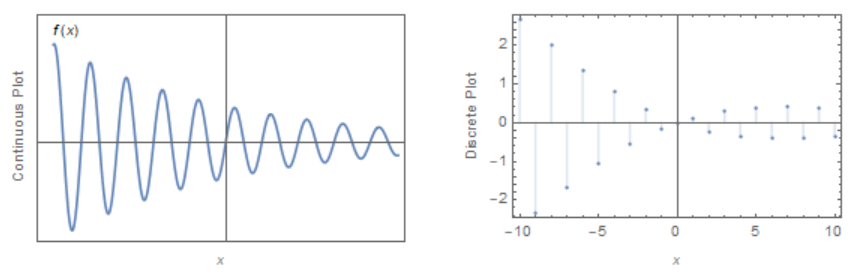
\includegraphics[height=0.4\textheight,keepaspectratio]{mathplot.png}
		\caption{خروجی قطعه کد فوق}
	\end{figure}
	
	\subsection{انجام دهید!}
	سیگنال‌های زیر را در بازه‌ی زمانی $-5 \le t \le 5$ رسم کنید. (توزیع ضربه را باید خودتان تعریف کنید، دامنه‌ی آن را برای راحتی واحد در نظر بگیرید)
	\begin{latin}
		\begin{flushleft}
			\begin{enumerate}
				\item $x_1(t) = sinc(t)$
				\item $x_2(t) = u(t+1) - u(t-1)$
				\item $x_3(t) = \begin{cases}
									0, & t < -1,\\
									1, & -1 < t < 0\\
									e^{-\nicefrac{t}{2}}, & 0 < t.
								\end{cases}$
				\item $x_4(t) = \delta(t-3) + 2\delta(t+1)$
				\item $x_5(t) = Standard Gaussian Function$
			\end{enumerate}
		\end{flushleft}
	\end{latin}

	\subsection{انجام دهید!}
	دو تابع انرژی و توان را طوری بنوسید که یک سیگنال را به عنوان ورودی بگیرد و انرژی یا توان آن را گزارش کند. انرژی و توان سیگنال‌های فوق را در قالب \lstinlint{Table} گزارش کنید. مقادیر بدست آمده را با تحلیل دستی خود مقایسه کنید.
	\subsection{انجام دهید!}
	مقدار \lstinline{DC} توابع قسمت ۲.۲ را نیز محاسبه کرده و در قالب \lstinlint{Table}  ارائه دهید. مقادیر بدست آمده را با تحلیل دستی خود مقایسه کنید.
	\subsection{انجام دهید!}
	می‌خواهیم برای پردازش‌های بعدی از سیگنال زیر نمونه‌برداری کنیم. برای این که ابتدا سیگنال را تعریف کرده سپس آن را در بازه‌ی $-5 \le t \le 5$ رسم کنید.
	$$x_6(t) = sin(t) + 0.5 sin(3t)$$
	نمونه‌برداری به این صورت است که تابع ضربه‌ای را از چپ به راست حرکت داده و در سیگنال مورد نظر ضرب می‌کنیم.
	$$x_s(t) = x(t)\delta_T_s(t) = \sum_{n} x(nT_s)\delta(t-nT_s)$$
	برای این کار، از تابع ضربه‌ای که برای رسم قسمت ۲.۲ از آن استفاده کردید کمک بگیرید. همچنین کافی است این ضرب را در بازه‌ی $-5 \le t \le 5$ و با فاصله‌های $0.1$ انجام داده، نتایج را در یک \lstinline{Table} ذخیره کنید، سپس شکل حاصل را رسم کنید. شکل حاصل باید مشابه شکل زیر باشد.
	\begin{figure}[h]
		\centering
		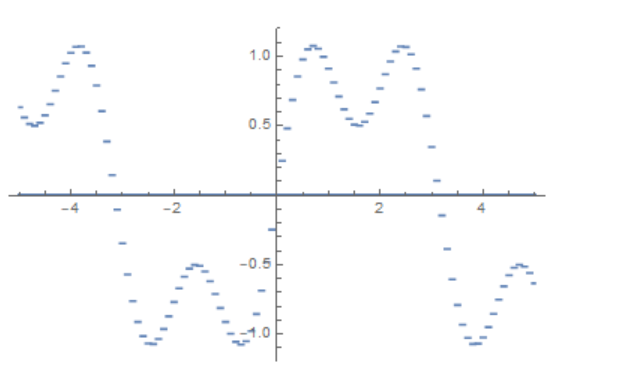
\includegraphics[height=0.3\textheight,keepaspectratio]{sample.png}
		\caption{سیگنال پس از نمونه‌برداری}
	\end{figure}
	
	\section{آشنایی با متلب}
	\subsection{کانولوشن گسسته-زمان}
	کانولوشن دو سیگنال گسسته $x[n]$ و $h[n]$ به صورت زیر تعریف می‌شود:
	$$y[n]=\sum_{m=-\infty}^{+\infty} x[m]h[n-m]$$
	تصویری از تعریف بالا را می‌توان به این صورت شرح داد: ابتدا دنباله  $h[m]$ نسبت به محور عمودی منعکس می‌شود و  $n$ نمونه به سمت چپ یا راست (با توجه به علامت $n$) جابجا می‌شود. سپس دنباله  $h[n-m]$ در دنباله  $x[m]$ ضرب می‌شود و حاصل‌جمع ِدنباله حاصل را بدست می‌آوریم. این تصویر از ویژگی خطی بودن و تغییر ناپذیری زمان سیستم های گسسته-زمان بدست می‌آید. در این قسمت استفاده از تابع \lstinline[language=Octave]{conv} (در پایتون \lstinline[language=Python]{numpy.convolve}) را یاد می‌گیرید.
	\subsection{آموزش \lstinline[language=Octave]{conv}}
	اگر فرض کنیم سیگنال $x[n]$ فقط در بازه‌ای به طول $N_x$ و سیگنال $h[n]$ فقط در بازه‌ای به طول $N_h$ مقدار غیر صفر داشته باشند، آنگاه سیگنال $y[n]$ فقط در بازه‌ای بطول $N_x+N_h-1$ غیر صفر خواهد بود. بدین معنی که اگر  \lstinline[language=Octave]{x} برداری $N_x$ بعدی شامل مقادیر سیگنال  $x[n]$ و \lstinline[language=Octave]{h} برداری $N_h$ بعدی شامل مقادیر سیگنال $h[n]$ باشد، دستور 
	\begin{latin}
		\lstinputlisting[language=Octave]{convhx.m}
	\end{latin}
	\noindent به تعداد $N_x+N_h-1$ نمونه از $y[n]$ را در بردار \lstinline[language=Octave]{y} برمی‌گرداند.
	
	اگر دقت کرده باشبد، این دستور هیچ اطلاعی در مورد اندیس زمانی نمونه‌های سیگنال $y[n]$ (که در بردار \lstinline[language=Octave]{y} ذخیره شده است) برنمی‌گرداند که مورد انتظار نیز هست. چون هیچ ورودی از اندیس بردارهای \lstinline[language=Octave]{x} و \lstinline[language=Octave]{h} نمی‌گیرد. در این حالت باید خودتان اندیس‌‌های مناسبی بسازید. در ادامه با مثالی ساده نحوه‌ی ساخت این اندیس‌ها را یاد می‌گیرید.
	
	سیگنال زیر با طول محدود را در نظر بگیرید:
	$$
	x[n]=\begin{cases}
		1, & 0 \le n \le 5,\\
		0, & \text{otherwise}.
	\end{cases}
	$$
	ابتدا حاصل عبارت $y[n]=x[n]*x[n]$ را با تحلیل دستی حساب کنید.
	
	به کمک کد زیر می‌توانید کانولوشن را حساب کرده و آن را رسم کنید. دقت کنید که باید تابع \lstinline[language=Octave]{convIndices} را پیاده سازی کنید.
	\begin{latin}
		\lstinputlisting[language=Octave]{conv_example.m}
	\end{latin}
	
	\subsection{انجام دهید!}
	در این قسمت تابع \lstinline[language=Octave]{convIndices} را پیاده‌سازی می‌کنید.
	
	برای بدست آوردن بردار \lstinline[language=Octave]{ny} دو سیگنال زیر را در نظر بگیرید:
	\begin{align*}
	h[n] &= \delta[n - a] + \delta[n - b],\\
	x[n] &= \delta[n - c] + \delta[n - d].
	\end{align*}
	با تحلیل دستی $y[n]=x[n]*x[n]$ را حساب کنید. سپس \lstinline[language=Octave]{ny} را بر حسب $a$، $b$، $c$ و $d$ تعیین کنید. حال می‌توانید تابع  \lstinline[language=Octave]{convIndices} را بنویسید. این تابع اندیس زمانی ورودی‌های کانولوشن را ورودی می‌گیرد و اندیس زمانی مناسبی برای خروجی کانولوشن می‌دهد. در این مثال ورودی های این تابع دو بردار به صورت \lr{\lstinline[language=Octave]{nh = a : b}} و \lr{\lstinline[language=Octave]{nx = c : d}} هستند.
	\subsection{انجام دهید!}
		سیگنال ورودی $x[n]$ و پاسخ ضربه ضربه $h[n]$ به صورت زیر تعریف شده‌اند:
		\begin{align*}
			x[n] &= \left(\frac{1}{2}\right)^{n-2}u[n-2],\\
			h[n]‌&= u[n]
		\end{align*}
		حال اگر بخواهید $y[n]=h[n]*x[n]$ را با دستور \lstinline[language=Octave]{conv} حساب کنید، باید ملاحظاتی برای طول بی‌نهایت دو سیگنال $x[n]$ و $h[n]$ بکنید.
		
		مقادیر $x[n]$ در بازه‌ی $0\le n\le24$ را در بردار \lstinline[language=Octave]{x} و مقادیر $h[n]$ در بازه‌ی $0\le n\le14$ را در بردار \lstinline[language=Octave]{h} ذخیره کنید. حال حاصل کانولوشن این دو سیگنال را در بردار \lstinline[language=Octave]{y} ذخیره کنید. این در حالی است که شما فقط قسمتی از دو سیگنال $x[n]$ و $h[n]$ را در نظر گرفته‌اید. پس فقط بخشی از سیگنال خروجی دارای مقادیر درست است.
		
		مقادیر $a$، $b$، $c$ و $d$ را به نحوی که \lr{\lstinline[language=Octave]{nh = a : b}} و \lr{\lstinline[language=Octave]{nx = c : d}} باشند، تعیین کنید و از جواب قسمت قبل برای بدست آوردن \lstinline[language=Octave]{ny} استفاده کنید. با دستور \lstinline[language=Octave]{stem} سیگنال $y[n]$ را رسم کنید و مشخص کنید چه بخشی از مقادیر آن با ارزش و چه بخشی بی‌ارزش است. (از برچسب‌های مناسب برای نمایش سیگنال خروجی استفاده کنید.)
	\subsection{انجام دهید!}
	تابع کانولوشن را خودتان پیاده سازی کنید و آن را \lstinline[language=Octave]{myConv} بنامید.
	سیستمی با پاسخ ضربه‌ی زیر فرض کنید:
	$$
	h[n] = sinc(2\pi n) (u[n + 4] - u[n - 5])
	$$
	خروجی این سیستم را یکبار با تابع کانولوشن متلب و یکبار با تابع خوتان برای ورودی زیر حساب کنید و صحت تابع خود را بررسی کنید.
	$$
	x[n]=u[n]-n[n-2]
	$$
	با دستور \lstinline[language=Octave]{tic} و \lstinline[language=Octave]{toc} مدت زمان انجام کانولوشن خودتان و کانولوشن متلب را بدست آورید و مقایسه کنید. علت اختلاف را شرح دهید.
	\subsection{انجام دهید (امتیازی)!}
	در این قسمت می‌خواهیم از روش کانولوشن بلوکی استفاده کنیم. این روش در پیاده سازی بی‌درنگ فیلترهای دیجیتال برای پردازش صوت/تصویر استفاده می‌شود.

	در این روش سیگنال ورودی (که سیگنالی با طول بی‌نهایت/نامعلوم است) را به بلوک‌های کوچکتر تقسیم می‌کنیم. حال می‌توانیم هر کدام از این بلوک‌ها را به صورت مستقل پردازش کنیم البته با کمی تأخیر. 
	
	خطی بودن کانولوشن این تضمین را می‌دهد که برهم‌نهی \LTRfootnote{Superposition} خروجی‌های حاصل از پردازش بلوک‌ها با کانولوشن کل سیگنال با پاسخ ضربه یکسان است. وجود سخت افزار با کارایی مناسب و الگوریتم‌‌هایی برای محاسبه کانولوشن سیگنال‌هایی با طول محدود، بر اهمیت روش کانولوشن بلوکی ‌می‌افزاید. در این قسمت هر کدام از کانولوشن‌های کوچک را با دستور \lstinline[language=Octave]{conv} حساب می‌کنید.
	
	فرض کنید یک سیستم با پاسخ ضربه‌ی $h[n]$ دارید که فقط در بازه‌ی $0\le n \le P-1$ غیر صفر است. همچنین فرض کنید دنباله‌ی ورودی یعنی $x[n]$ برای $n<0$ صفر است و طول آن به طور قابل ملاحظه‌ای از $P$ بیشتر است.حال می‌توانید به صورت زیر سیگنال $x[n]$ را به بلوک‌هایی با طول $L$ تقسیم کنید:
	$$
	x[n] = \sum_{r=0}^{\infty}x_r[n-rL]
	$$
	که در آن $L>P$ و داریم:
	$$
	x_r[n]=\begin{cases}
		x[n+rL]&, 0 \le n \le L-1,\\
		0&, \text{(otherwise)}
	\end{cases}
	$$
	شکل زیر را ببینید:
	\begin{figure}[h]
		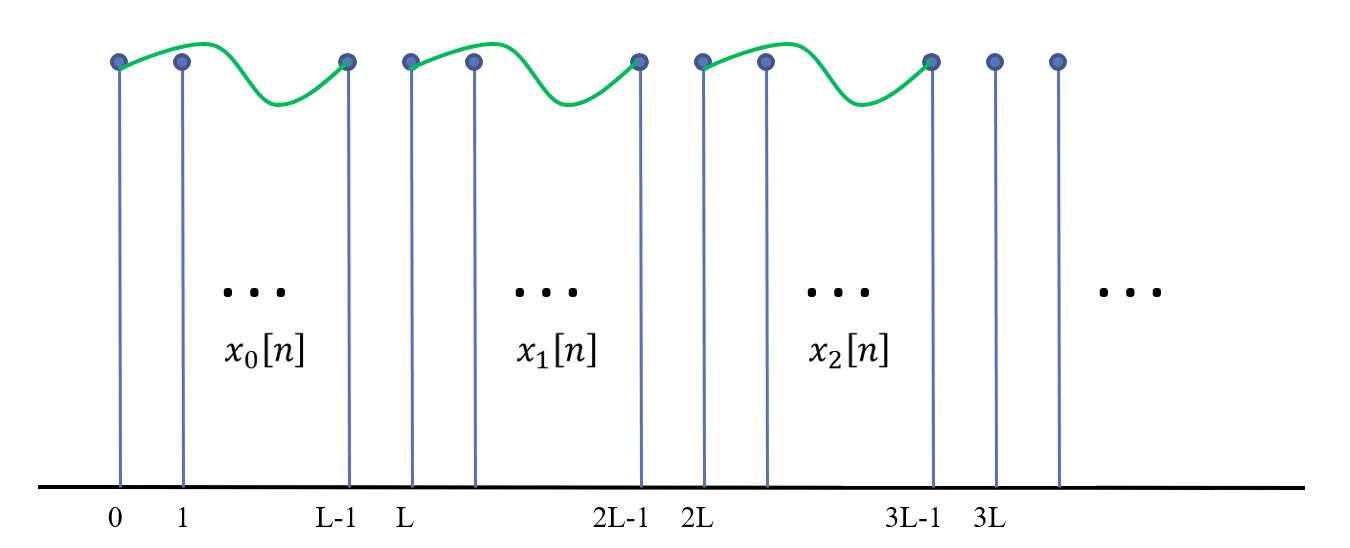
\includegraphics[width=\linewidth]{segments.png}
		\caption{تجزیه بلوکی سیگنال $x[n]$}
	\end{figure}
	
	ابتدا برای دو سیگنال زیر $y[n]=h[n]*x[n]$ را با دستور \lstinline[language=Octave]{conv}  در بازه‌ی $0\le n \le 99$ حساب کنید و نمودار آن را با \lstinline[language=Octave]{stem} در بازه‌ی داده شده رسم کنید.
	\begin{align*}
	x[n] &= cos(n^2)sin(2\pi n/5),\\
	h[n]‌&= (0.9)^n(u[n]-u[n-10])
	\end{align*}
	با فرض $L=50$ سیگنال $x[n]$ را به دو بلوک تقسیم کنید که طول هر کدام 50 شود. دو سیگنال $y_0[n]=h[n]*x_0[n]$ و $y_1[n]=h[n]*x_1[n]$ را که در آن $x_0[n]$ 50 نمونه اول $x[n]$ و $x_1[n]$ 50 نمونه دوم $x[n]$ است، حساب کنید. حال فرم سیگنال خروجی به صورت زیر خواهد بود:
	$$y[n]=x[n]*h[n] = y_0[n] + y_1[n-k]$$
	در عبارت بالا $k$ مناسب را بدست آورید. (دقت کنید که طول هر کدام از سیگنال های $y_0[n]$ و $y_1[n]$ باید $L+P-1$ باشد.) وقتی سیگنال $y_0[n]$ و $y_1[n]$ را با هم جمع می‌کنید، ناحیه‌ای وجود دارد که در آن مقادیر غیر صفر از دو سیگنال با هم جمع می‌شوند. به این خاطر به روش کانولوشن بلوکی، "هم‌پوشانی و اضافه کردن" نیز می‌گویند. سیگنال خروجی یعنی $y[n]$ را با اسنفاده از این روش حساب کنید و آن را در بازه $0\le n \le 99$ با استفاده از \lstinline[language=Octave]{stem} رسم کنید. آیا به همان نتیجه قبلی می‌رسید؟ نتایج را تحلیل کنید.
	
	در نهایت یک تابع بنویسید که عمل هم‌پوشانی و اضافه کردن را انجام دهد. ورودی‌های این تابع پاسخ ضربه (\lstinline[language=Octave]{h})، بردار ورودی سیستم (\lstinline[language=Octave]{x}) و طول هر بلاک (\lstinline[language=Octave]{L}) ات. طول بردار \lstinline[language=Octave]{x} دلخواه و طول هر بلاک یک عدد دلخواه بزرگتر از طول فیلتر است. حال قسمت قبل را با تابع خود دوباره انجام دهید.
	
\end{document}